\documentclass[tikz,border=6pt]{standalone}
\usepackage{fontspec}
\usepackage{newtxmath}
\usepackage{bm}
\usepackage{tikz}
\definecolor{sfgreen}{RGB}{176,201,153}
\usetikzlibrary{calc,arrows.meta}
\newcommand{\err}[1]{\,\ensuremath{\bm{\mathit{\scriptscriptstyle #1}}}}  \setmainfont{Times New Roman}
\setmainfont{Times New Roman}

\begin{document}
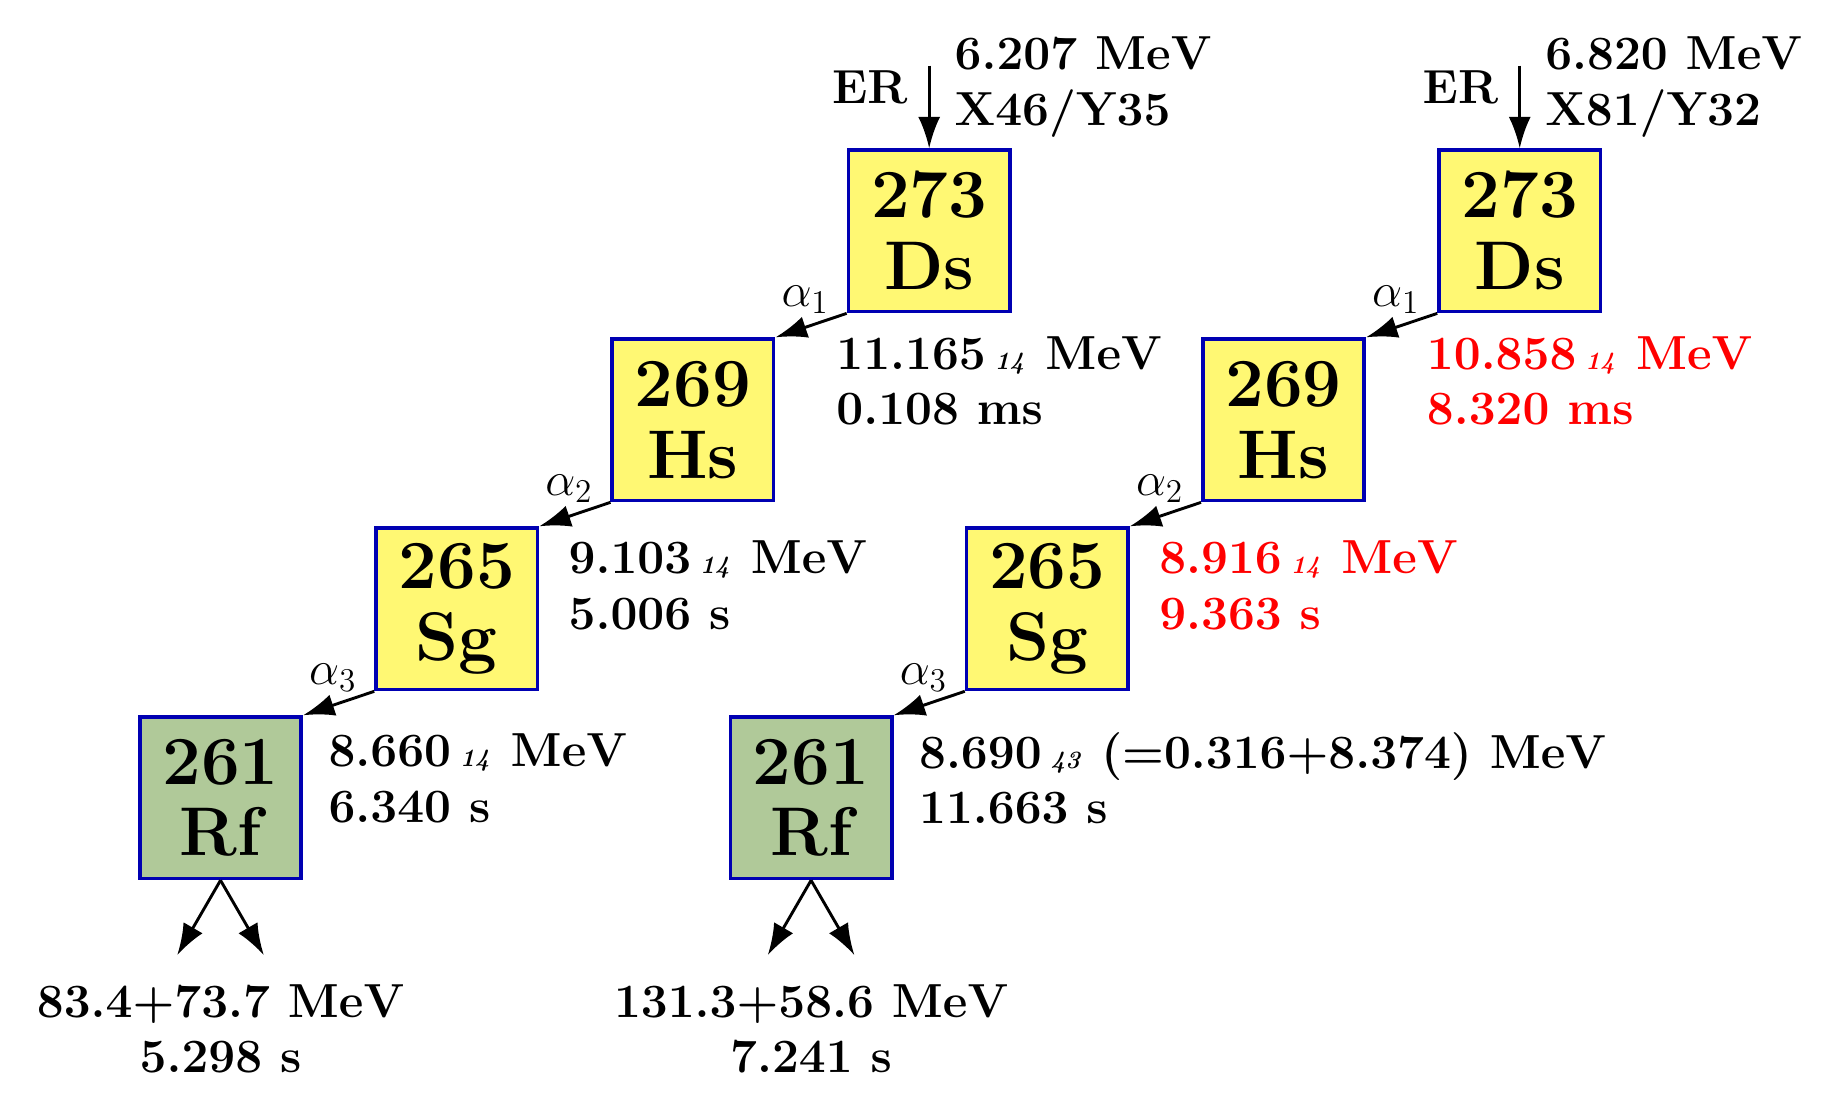
\begin{tikzpicture}[x=1cm,y=1cm]


% 样式
\tikzset{
  nucY/.style={
    draw=blue!70!black,
    line width=1.3pt,
    fill=yellow!55,
    minimum width=2.05cm,
    minimum height=2.05cm,
    align=center,
    inner sep=2pt,
    font=\bfseries\fontsize{24}{26}\selectfont
  },
  nucO/.style={
    draw=blue!70!black,
    line width=1.3pt,
    fill=orange!35,
    minimum width=2.05cm,
    minimum height=2.05cm,
    align=center,
    inner sep=2pt,
    font=\bfseries\fontsize{24}{26}\selectfont
  },
  arr/.style={
    -{Latex[length=4.0mm,width=2.8mm]},
    line width=1.05pt,
    draw=black
  },
  lbl/.style={
    font=\bfseries\fontsize{18}{20}\selectfont,
    text=black
  },
  blk/.style={
    font=\bfseries\fontsize{18}{20}\selectfont,
    text=black,
    align=left
  },
  redtxt/.style={
    font=\bfseries\fontsize{18}{20}\selectfont,
    text=red,
    align=left
  }
}

%--------------------------------
% 左链坐标
%--------------------------------
\node[nucY] (ds1) at (6.8,5.7) {273\\Ds};
\node[nucY] (hs1) at (3.8,3.3) {269\\Hs};
\node[nucY] (sg1) at (0.8,0.9) {265\\Sg};
\node[nucO,fill=sfgreen] (rf1) at (-2.2,-1.5) {261\\Rf};

%--------------------------------
% 右链坐标
%--------------------------------
\node[nucY] (ds2) at (14.3,5.7) {273\\Ds};
\node[nucY] (hs2) at (11.3,3.3) {269\\Hs};
\node[nucY] (sg2) at (8.3,0.9) {265\\Sg};
\node[nucO,fill=sfgreen] (rf2) at (5.3,-1.5) {261\\Rf};

%--------------------------------
% ER 向下箭头
%--------------------------------
\draw[arr] ($(ds1.north)+(0,1.05)$) -- (ds1.north);
\node[lbl,anchor=east] at ($(ds1.north)+(-0.15,0.78)$) {ER};
\node[blk,anchor=west] at ($(ds1.north)+(0.20,0.78)$) {6.207 MeV\\X46/Y35};

\draw[arr] ($(ds2.north)+(0,1.05)$) -- (ds2.north);
\node[lbl,anchor=east] at ($(ds2.north)+(-0.15,0.78)$) {ER};
\node[blk,anchor=west] at ($(ds2.north)+(0.20,0.78)$) {6.820 MeV\\X81/Y32};

%--------------------------------
% alpha 衰变箭头（更长）
%--------------------------------
\draw[arr] (ds1.south west) -- (hs1.north east);
\node[lbl] at ($(ds1.south west)!0.58!(hs1.north east)+(0.00,0.35)$) {$\alpha_1$};

\draw[arr] (hs1.south west) -- (sg1.north east);
\node[lbl] at ($(hs1.south west)!0.58!(sg1.north east)+(0.00,0.35)$) {$\alpha_2$};

\draw[arr] (sg1.south west) -- (rf1.north east);
\node[lbl] at ($(sg1.south west)!0.58!(rf1.north east)+(0.00,0.35)$) {$\alpha_3$};

\draw[arr] (ds2.south west) -- (hs2.north east);
\node[lbl] at ($(ds2.south west)!0.58!(hs2.north east)+(0.00,0.35)$) {$\alpha_1$};

\draw[arr] (hs2.south west) -- (sg2.north east);
\node[lbl] at ($(hs2.south west)!0.58!(sg2.north east)+(0.00,0.35)$) {$\alpha_2$};

\draw[arr] (sg2.south west) -- (rf2.north east);
\node[lbl] at ($(sg2.south west)!0.58!(rf2.north east)+(0.00,0.35)$) {$\alpha_3$};

%--------------------------------
% 左链文字
%--------------------------------
\node[blk,anchor=west] at ($(hs1.east)+(0.65,0.50)$) {11.165\err{14} MeV\\0.108 ms};
\node[blk,anchor=west]    at ($(sg1.east)+(0.25,0.30)$) {9.103\err{14} MeV\\5.006 s};
\node[blk,anchor=west]    at ($(rf1.east)+(0.20,0.25)$) {8.660\err{14} MeV\\6.340 s};

%--------------------------------
% 右链文字
%--------------------------------
\node[redtxt,anchor=west] at ($(hs2.east)+(0.65,0.50)$) {10.858\err{14} MeV\\8.320 ms};
\node[redtxt,anchor=west]    at ($(sg2.east)+(0.25,0.30)$) {8.916\err{14} MeV\\9.363 s};
\node[blk,anchor=west]    at ($(rf2.east)+(0.20,0.25)$) {8.690\err{43} (=0.316+8.374) MeV\\11.663 s};

%--------------------------------
% 底部分叉箭头
%--------------------------------
\draw[arr] (rf1.south) -- ($(rf1.south)+(-0.55,-0.95)$);
\draw[arr] (rf1.south) -- ($(rf1.south)+( 0.55,-0.95)$);
\node[font=\bfseries\fontsize{18}{20}\selectfont, text=black, align=center, anchor=north]
at ($(rf1.south)+(0,-1.20)$) {83.4+73.7 MeV\\5.298 s};



\draw[arr] (rf2.south) -- ($(rf2.south)+(-0.55,-0.95)$);
\draw[arr] (rf2.south) -- ($(rf2.south)+( 0.55,-0.95)$);
\node[font=\bfseries\fontsize{18}{20}\selectfont, text=black, align=center, anchor=north]
at ($(rf2.south)+(0,-1.20)$) {131.3+58.6 MeV\\7.241 s};

\end{tikzpicture}
\end{document}